\documentclass[border=10pt]{standalone}
\usepackage{pgfplots}
\begin{document}
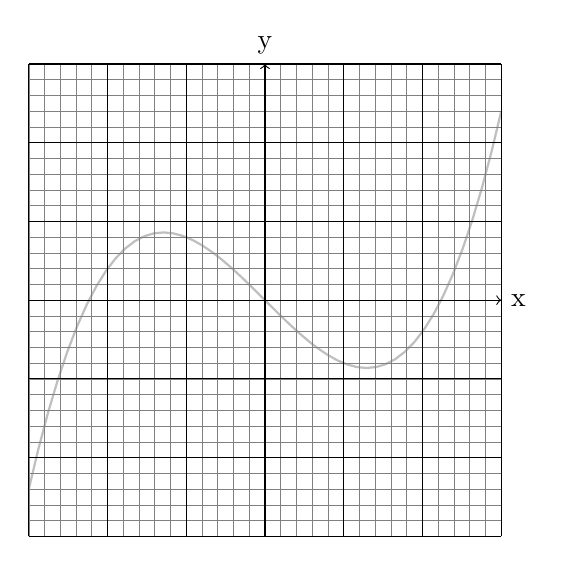
\begin{tikzpicture}
  \draw[domain=-3:3,samples=50,color=gray!50,thick] plot (\x, \x^3/5 - \x);
  \draw[very thin,gray,step=.2] (-3,-3) grid (3,3);
  \draw[step=1] (-3,-3) grid (3,3);
  \draw[->] (-3,0) -- (3,0) node[right] {x};
  \draw[->] (0,-3) -- (0,3) node[above] {y};
\end{tikzpicture}
\end{document}
